%!TEX root = main.tex
\documentclass[main.tex]{subfiles}

\begin{document}
This implementation was done in different phases. First came the purchasing of parts, then came their configuration, and then their connection. After this, the implementation of the filtration methods. Finally, all the information was configured to be displayed after the implementation of a UI.

\section{Raspberry Pi}
\subsection{OS}
After acquiring the Raspberry Pi 3, the first step was to install an operating system (OS). The research on RasPBX \cite{raspbx} mean that it was the chosen OS. The image was flashed to an SD card for the Raspberry Pi. There is no need for further details of this step.

\subsection{Network Connections}
The next step was to configure the Raspberry Pi 3 to act as a DHCP server \cite{pi-dhcp}, as the online resource suggested. Again, no further details are included as the instructions were followed. The Pi has created its own LAN, and assigns itself the address $192.168.3.1$. This allowed the Obi110 to be connected to the network through the switch.

\section{ObiHai Obi110 and the Phone}
As there is no landline in College to use, the Obi110 was brought home. Combined with a simple standard analogue phone, everything was connected to show that without any additional configuration, the normal phone with the Obi110 works normally. The only trouble was that the Obi110 was designed for American phone sockets, which meant a UK-US and a UK-US adapter was needed.

\section{Asterisk, FreePBX, and the Obi110}
This segment was done using a combination of materials from Bryan Ross \cite{bryanross}, and a little bit from Phil's Blog \cite{obihaiuk}. Ross's tutorial \cite{bryanross} allows RasPBX to interface with the phone line, and the analogue phone. The manipulation of the Obi110 settings was done through its web interface. RasPBX has an Asterisk server running, but has the FreePBX GUI that is accessible through the web as well. Although the steps that were followed were quite similar, they were only followed until the Obi110 and the RasPBX were linked. Ross's material continues to show how he did his time-based system, which is not relevant in this case.
\\\\
Before looking at the configuration, Figure \ref{fig:physical} shows how the components are laid out and how they are physically connected.

\begin{figure}[p]
\centering
\captionsetup[subfigure]{position=b}
	\begin{subfigure}{\textwidth}
		\centering
	\begin{tikzpicture}[node distance=4cm]
	    % We start by placing the blocks
		\node [input, align=center] (line) {Landline};
		\node [block, align=center, right of=line] (obi) {Obi110};
		\node [block, align=center, right of=obi] (phone) {Analogue\\Phone};
		\node [block, align=center, below of=obi] (power) {Power\\Source};
		\node [block, align=center, right of=power] (button) {Handset\\Button};
		\node [block, align=center, below of=button] (pi) {Raspberry\\Pi};
		\node [block, align=center, below of=power] (switch) {Switch};

	    % Once the nodes are placed, connecting them is easy.
	    \draw [<->] (line) -- node[align=center] {} (obi);
		\draw [<->] (obi) -- node[align=center] {} (phone);
		\draw [<->] (phone) -- node[align=center] {} (button);
		\draw [<->] (button) -- node[align=center] {} (pi);
		\draw [->] (power) -- node[align=center] {} (obi);
		\draw [->] (power) -- node[align=center] {} (pi);
		\draw [->] (power) -- node[align=center] {} (switch);
		\draw [<->] (pi) -- node[align=center] {} (switch);
		\draw [<->] (obi.south west) to [bend right=90] node[align=center, above] {} (switch.west);

	\end{tikzpicture}
	\caption{Physical connections of the system.}
	\label{fig:physical-diagram}
\end{subfigure}
\\
\begin{subfigure}{\textwidth}
	\centering
	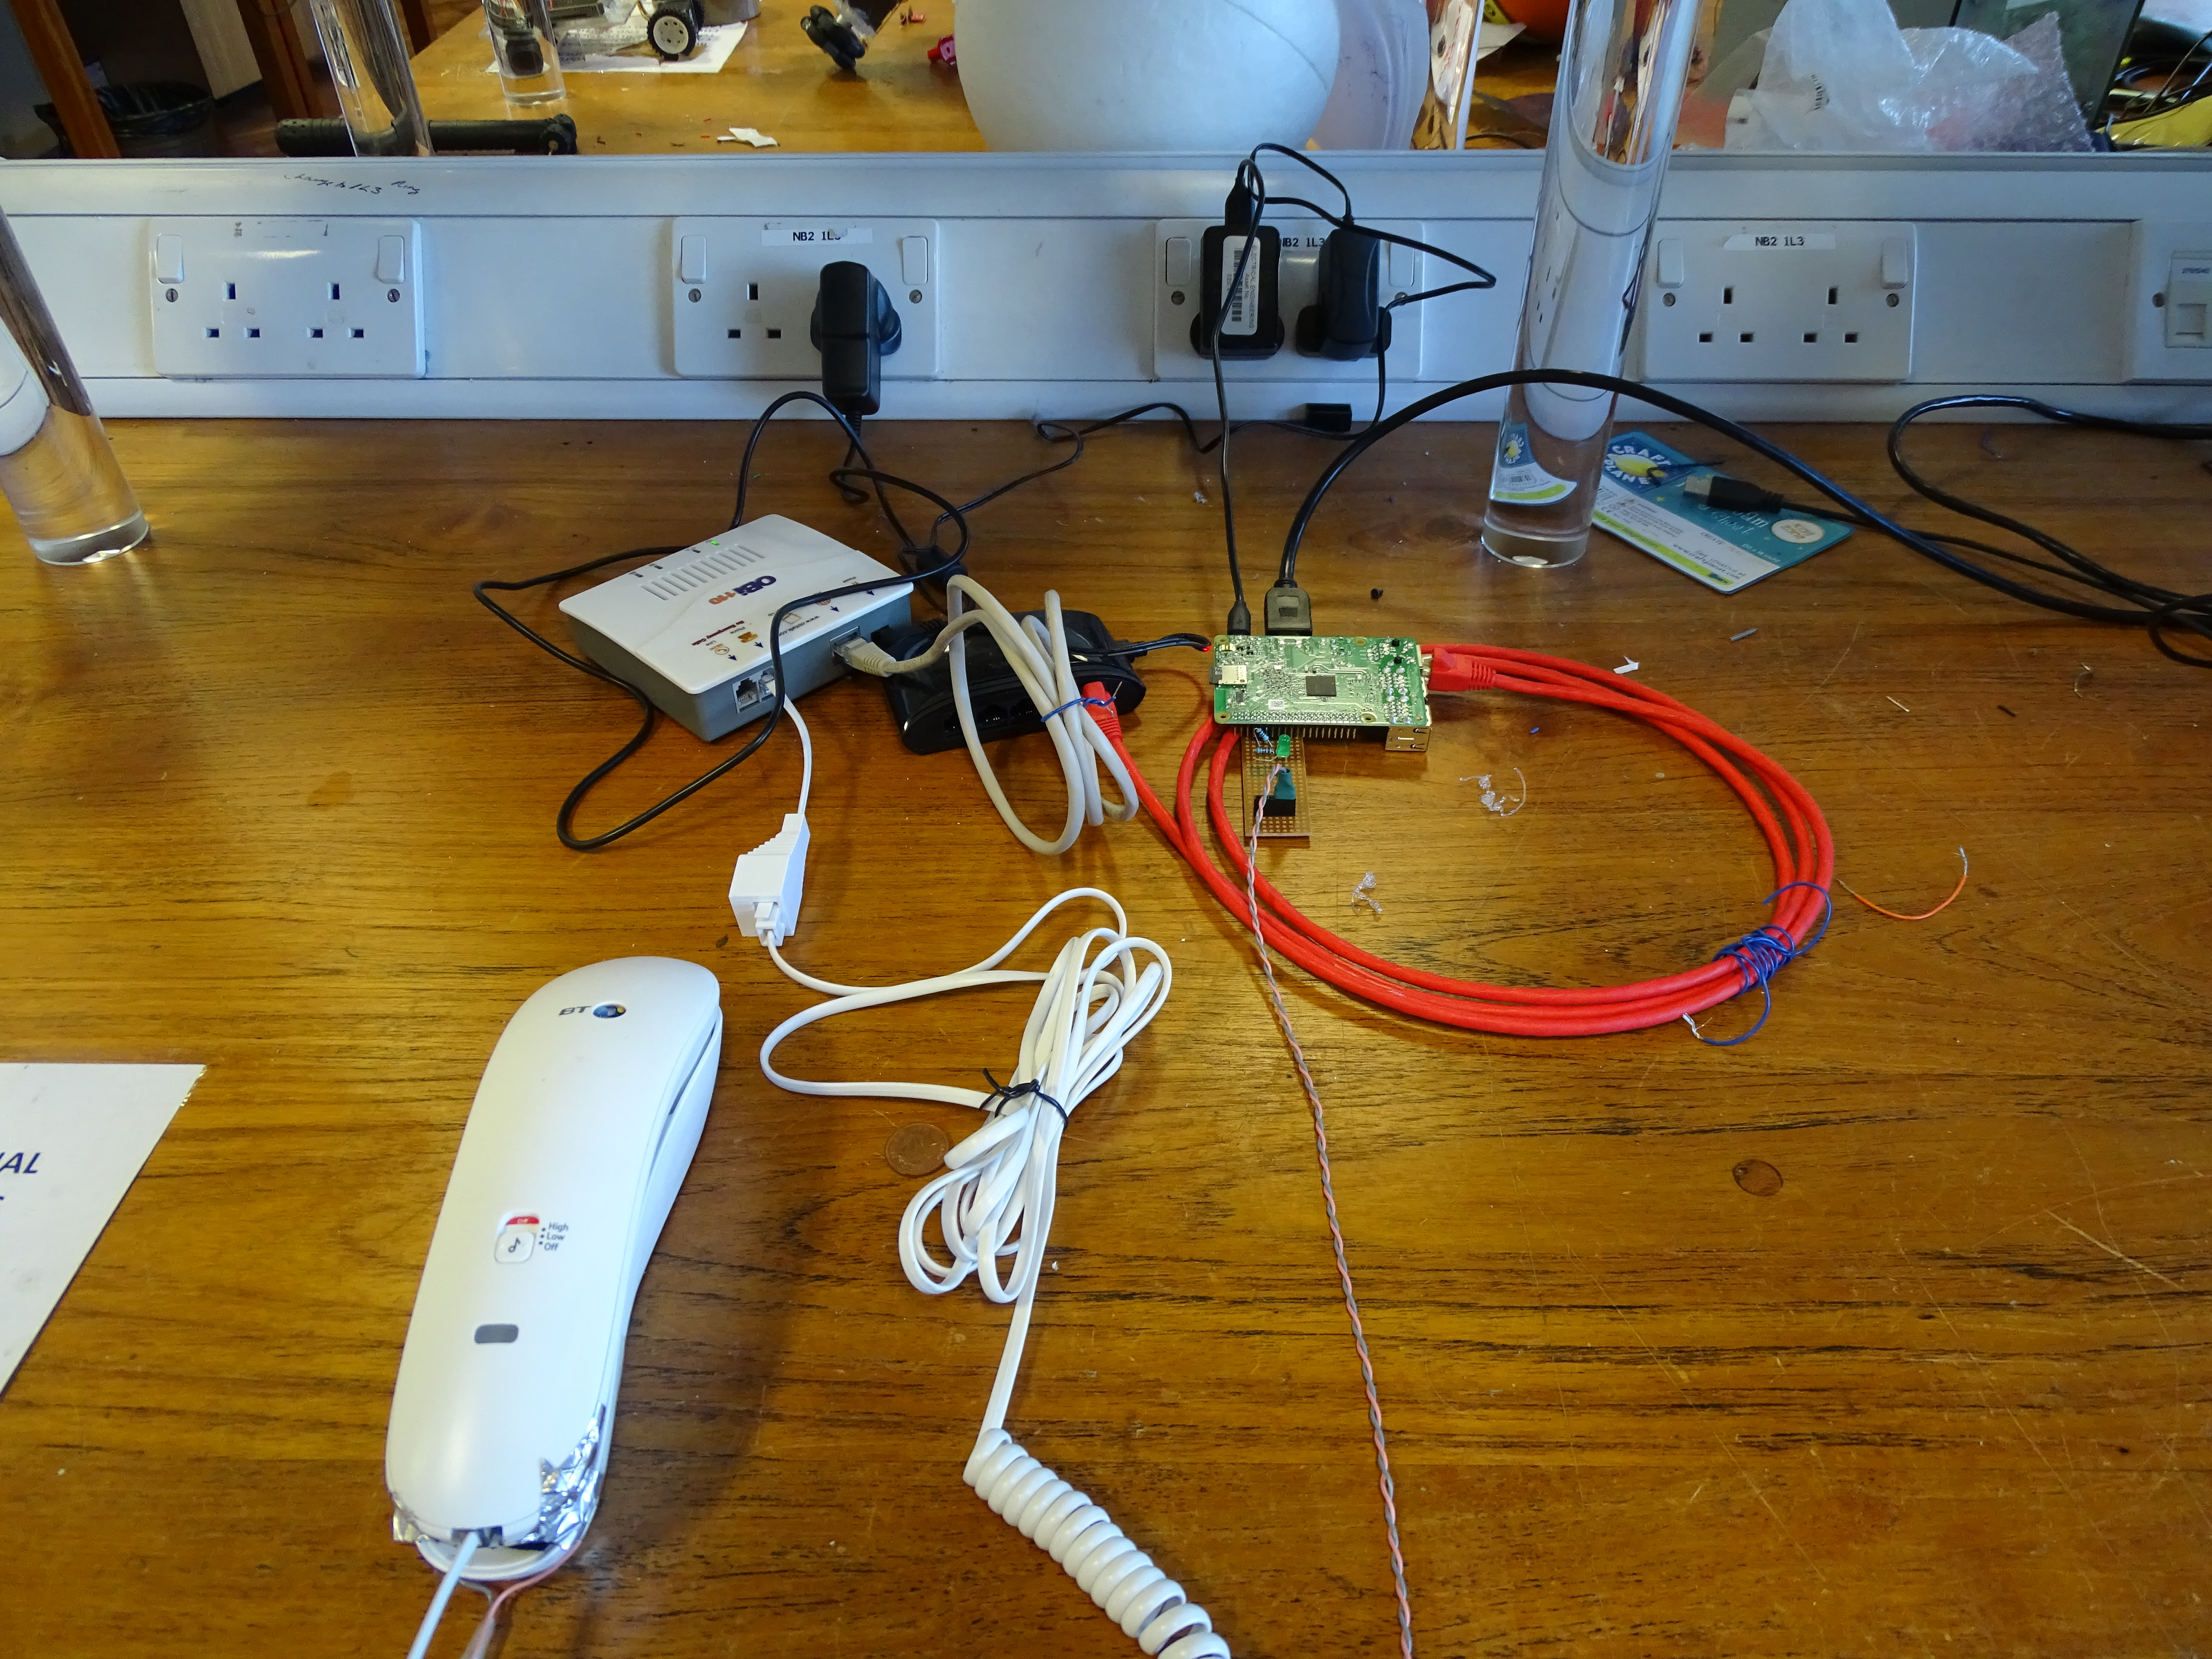
\includegraphics[width=0.8\textwidth]{pics/meng/setup}
	\caption{A picture of everything.}
	\label{fig:physical-picture}
\end{subfigure}
\caption{The layout of the implementation, both in block diagram, and with a picture. }
\label{fig:physical}
\end{figure}

To briefly summarise the settings, the first thing is that the Obi110 is able to ``convert'' the landline into an SIP trunk. This trunk is what Asterisk can use to send and receive calls from the outside. This ensures that calls going to the trunk from Asterisk are converted into something the landline can handle, while calls coming in are sent to the trunk.
\\\\
Next, the Obi110's interface with the analogue telephone is configured as an extension. An extension in this context is an endpoint in a VoIP system. In other words, by configuring it as an extension, it can receive calls sent to it from Asterisk, and will convert it into a form that the phone can handle. Phil's Blog contained some important configuration values that were used to ensure a smoother calling process \cite{obihaiuk}. The entire Obi110 configuration is stored as an XML file, which is included in the repository, a link to which can be found in Appendix \ref{sec:appendix-repo} as it is relevant, but not necessary in the main body.
\\\\
Once this is done, the Asterisk server was configured through the FreePBX GUI. The server was set to interact with the trunk from the Obi110. This would be where all outbound calls are headed. Next, all inbound calls would be routed to the analogue phone extension in the Obi110. This means that calls headed out go through the SIP trunk to the landline, and incoming calls go straight to the phone.
\\\\
At this point, all the connections to the outside are configured and set. While an additional VoIP phone was obtained from the department, the proprietary nature of the phone meant that it was not possible to use it with the open-source software that was running on the Raspberry Pi. The configuration flow inside is shown in Figure \ref{fig:asterisk-conf}.

\begin{figure}[p]
	\captionsetup[subfigure]{position=b}
        \centering
        \begin{subfigure}{\textwidth}
			\centering
			\begin{tikzpicture}[node distance=5cm]
			% We start by placing the blocks
			\node [input, align=center] (input) {Output\\to\\Landline};
			\node [output, align=center, below of=input] (output) {From\\Phone};
			\node [block, align=center, right of=input] (converter1) {Landline\\to\\SIP\\Conversion};
			\node [block, align=center, right of=output] (converter2) {SIP\\to\\Landline\\Conversion};
			\node [inner sep=7pt, draw,thick,fit=(converter1) (converter2)] (obi) {Obi110};
			\node [block, align=center, right of=converter1] (inboundrules) {Outbound\\Rules};
			\node [block, align=center, right of=converter2] (ext) {Origin\\Extension};
			\node [inner sep=15pt, draw,thick,fit=(inboundrules) (ext), label={Asterisk}] (ast) {};

			% Once the nodes are placed, connecting them is easy.
			\draw [draw,<-] (input) -- node[align=center] {} (converter1);
			\draw [->] (output) -- node[align=center] {} (converter2);
			\draw [<-] (converter1) -- node[align=center, above] {Trunk} (inboundrules);
			\draw [<-] (inboundrules) -- node[align=center, right] {Call\\Routing} (ext);
			\draw [<-] (ext) -- node[align=center] {} (converter2);

		\end{tikzpicture}
		\caption{Internal Asterisk call routing setup for outgoing calls.}
		\label{fig:asterisk-conf-out}
        \end{subfigure}
        \\
        \begin{subfigure}{\textwidth}
			\centering
			\begin{tikzpicture}[node distance=5cm]
			    % We start by placing the blocks
			    \node [input, align=center] (input) {Input\\from\\Landline};
				\node [output, align=center, below of=input] (output) {To\\Phone};
			    \node [block, align=center, right of=input] (converter1) {Landline\\to\\SIP\\Conversion};
				\node [block, align=center, right of=output] (converter2) {SIP\\to\\Landline\\Conversion};
				\node [inner sep=7pt, draw,thick,fit=(converter1) (converter2)] (obi) {Obi110};
			    \node [block, align=center, right of=converter1] (inboundrules) {Inbound\\Rules};
				\node [block, align=center, right of=converter2] (ext) {Destination\\Extension};
				\node [inner sep=15pt, draw,thick,fit=(inboundrules) (ext), label={Asterisk}] (ast) {};

			    % Once the nodes are placed, connecting them is easy.
			    \draw [draw,->] (input) -- node[align=center] {} (converter1);
			    \draw [<-] (output) -- node[align=center] {} (converter2);
				\draw [->] (converter1) -- node[align=center, above] {Trunk} (inboundrules);
				\draw [->] (inboundrules) -- node[align=center, right] {Call\\Routing} (ext);
				\draw [->] (ext) -- node[align=center] {} (converter2);

			\end{tikzpicture}
			\caption{Internal Asterisk call routing setup for incoming calls.}
			\label{fig:asterisk-conf-in}
        \end{subfigure}
	\caption{Visualisations of the call flows in and out of the system by linking trunks, extensions, outbound rules, and inbound rules}
	\label{fig:asterisk-conf}
\end{figure}

\subsection{Message, Prompt, and Code}
However, according to Figure \ref{fig:callflow}, the incoming call must go to a Welcome message. This is what the Interactive Voice Response (IVR) was used. The incoming calls are routed to an instance of it. This instance contains a message, and reacts according to the input from the caller. By combining the Welcome message with the reverse Turing test, the process is simplified. The message that the caller hears is as follows.

\begin{quote}
	\textit{Welcome! This system is monitored using an anti-spam system. Marketing calls and illegal activity will not be tolerated. Please press 1 to continue.}
\end{quote}

If the caller knows the weakly secret code (another number, such as 4 or 9), then the call is routed directly to the analogue extension, without any further delays. If the caller fails to press 1, or the code, or does not react, the IVR directs the call to a recorded message as follows, before the call ends.

\begin{quote}
	\textit{Unfortunately, there was an incorrect response. Please redial this number and press 1 at the prompt. Thank you!}
\end{quote}

If the reverse Turing test is passed (i.e. ``1'' is pressed), then the IVR directs the call to a Call Recording module. While the neither the caller or the user sees this, the Call Recording module, which takes in a call and redirects to an extension, has begun recording the call. This is for the voice extraction, which is explained later.
\\\\
All of this is seen in Figure \ref{fig:asterisk-callflow}, which shows the call flow inside the server.

\begin{figure}[htb]
\centering
\resizebox{\textwidth}{!}{%
	\begin{tikzpicture}[node distance=4cm]
	    % We start by placing the blocks
		\node [input, align=center] (call) {Incoming\\Call};
		\node [block, align=center, right of=call] (ivr) {Welcome\\Message\\and IVR};
		\node [block, align=center, right of=ivr] (record) {Call\\Recording};
		\node [block, align=center, below of=record] (goodbye) {Goodbye\\Message};
		\node [block, align=center, right of=record] (ext) {Analogue\\Extension};
		\node [block, align=center, below of=ext] (end) {Call\\Ends};
		\node [output, align=center, right of=ext] (user) {User};

	    % Once the nodes are placed, connecting them is easy.
	    \draw [->] (call) -- node[align=center] {} (ivr);
	    \draw [->] (ivr) -- node[align=center, above] {Test\\passed} (record);
		\draw [->] (record) -- node[align=center] {} (ext);
		\draw [->] (ivr.south) |- node[align=center, left] {Test failed} (goodbye.west);
		\draw [->] (ext) -- node[align=center] {} (user);
		\draw [->] (goodbye) -- node[align=center] {} (end);
		\draw [->] (ivr) to [bend left=90] node[align=center, above] {Secret Code} (ext);

	\end{tikzpicture}%
	}
	\caption{Internal Asterisk call routing setup.}
	\label{fig:asterisk-callflow}
\end{figure}

\subsection{Voice Analysis}
In this section, the voice analysis method is implemented. This was done primarily in Python3 for the reason that it allows rapid development, and is extremely versatile. The versatility is highly valuable because it means the different components in this system can be manipulated with a single language, which allows information to be shared more easily. Prior familiarity with the language was also taken into account.

\subsubsection{Extraction of Voice}
The reason for the recording of the call is that it is a pre-existing feature that uses the available infrastructure to obtain the audio from the call. The addition of recording devices that need to be plugged-in to the phone worked against the Design Aims previous discussed in the Chapter \ref{chp:des}. The voice data is stored on the server, which allows for processing on the server itself. By polling the directory for new files, a Python script is able to locate the newly created file.

\begin{figure}[p]
	\captionsetup[subfigure]{position=b}
        \centering
        \begin{subfigure}{\textwidth}
                \includegraphics[width=\textwidth]{pics/wave1}
                \caption{Sample call recording visualised.}
                \label{fig:wave1}
        \end{subfigure}
        \\
        \begin{subfigure}{\textwidth}
                \includegraphics[width=\textwidth]{pics/wave2}
                \caption{Zoomed into the ringing signal.}
                \label{fig:wave2}
        \end{subfigure}
	\caption{Visualisations of the call data.}
	\label{fig:wave}
\end{figure}

It was at this point that the need for a switch was noticed. It was obvious that the recording would start the minute the call was put through. However, the recording included the initial ringing, and started before the user had picked up the phone. There was thus no way to determine how long since the user had picked up the phone. Looking at the waveform of the audio in Figure \ref{fig:wave}, it was seen that the ringing had a distinctive pattern, which could be easily identified. With the ringing happening at regular intervals, one method considered was to use a matched filter to the ringing and note its last instance. However, this was not just very involved, but also very computationally intensive.
\\\\
The switch as previous mentioned in the Design chapter was used. Conductive tape was connected to the receiver of the analogue phone, and two conductive pads were placed on the housing. When the phone was down, the tape closed the circuit, and when it was lifted off, the connection was broken. However, it was found that the voltage drop when the handset was removed was insufficient for the Pi to detect as a \texttt{LOW} value. Thus, a modification to the circuit was made by changing the $300\Omega$ resistor into 2 $150\Omega$ resistors in parallel. The switch then was made to short both the LED and one of the resistors, lowering the voltage detected by the Pi when it was open. This was found to be successful. The new circuit diagram is shown in Figure \ref{fig:newcircuit}, and Figure \ref{fig:button} contains pictures of the circuit connected to the Raspberry Pi, and the conductive tape layout on the handset.

\begin{figure}[h]
	\centering
	\begin{circuitikz} \draw
		 (0, 0) -- (8, 0)
		 (5, 0) to [R, l_=$150\Omega$] (5, 2)
		 (5, 2) to [R, l_=$150\Omega$] (5, 4)
		 (1, 2) node[label={above:To GPIO}] {} -- (5, 2)
		 (5, 6) to [led] (5, 4)
		 (3, 6) to [push button] (3, 2)
		 (0, 6) node[label={above:3.3V}] {} -- (8, 6)
		 (7, 0) node[ground]{} -- (7, 0)
		;
	\end{circuitikz}
	\caption{Modified switch circuit.} \label{fig:newcircuit}
\end{figure}
\vspace{-0.25cm}
\begin{figure}[h]
	\captionsetup[subfigure]{position=b}
        \centering
        \begin{subfigure}{0.47\textwidth}
                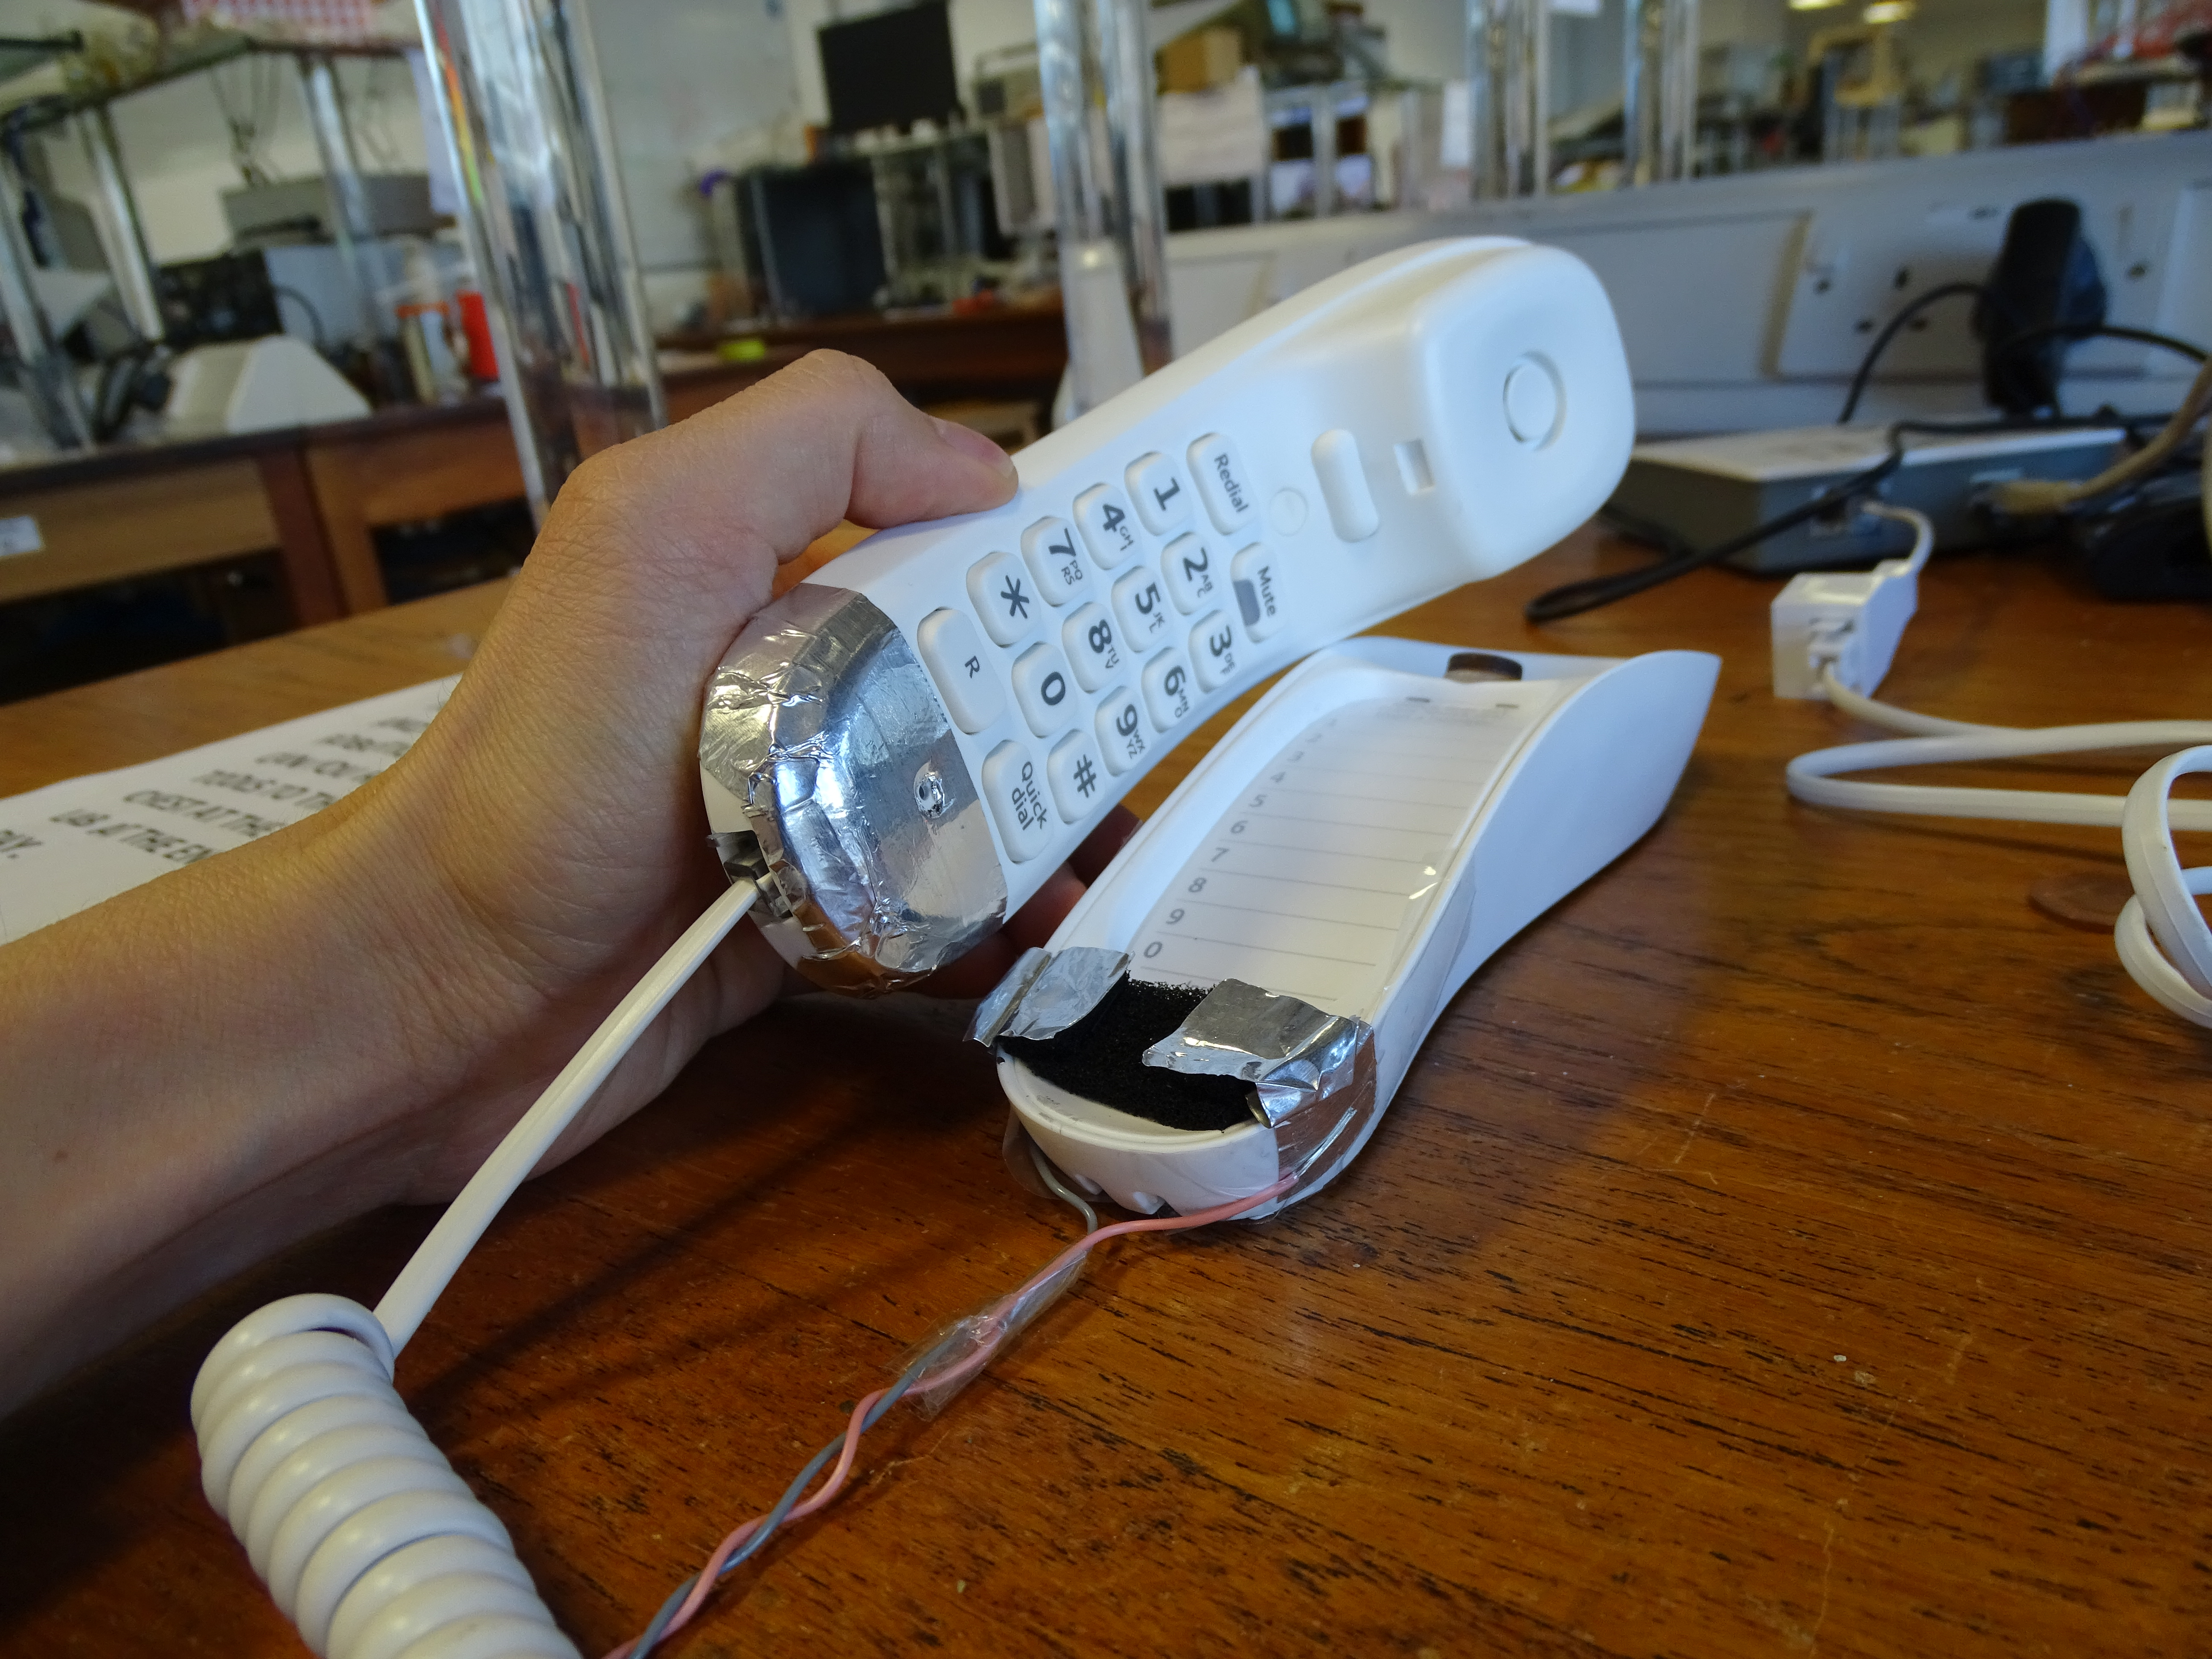
\includegraphics[width=\textwidth]{pics/meng/switch}
                \caption{Normal operation.}
                \label{fig:switch}
        \end{subfigure}
        ~
		\begin{subfigure}{0.47\textwidth}
                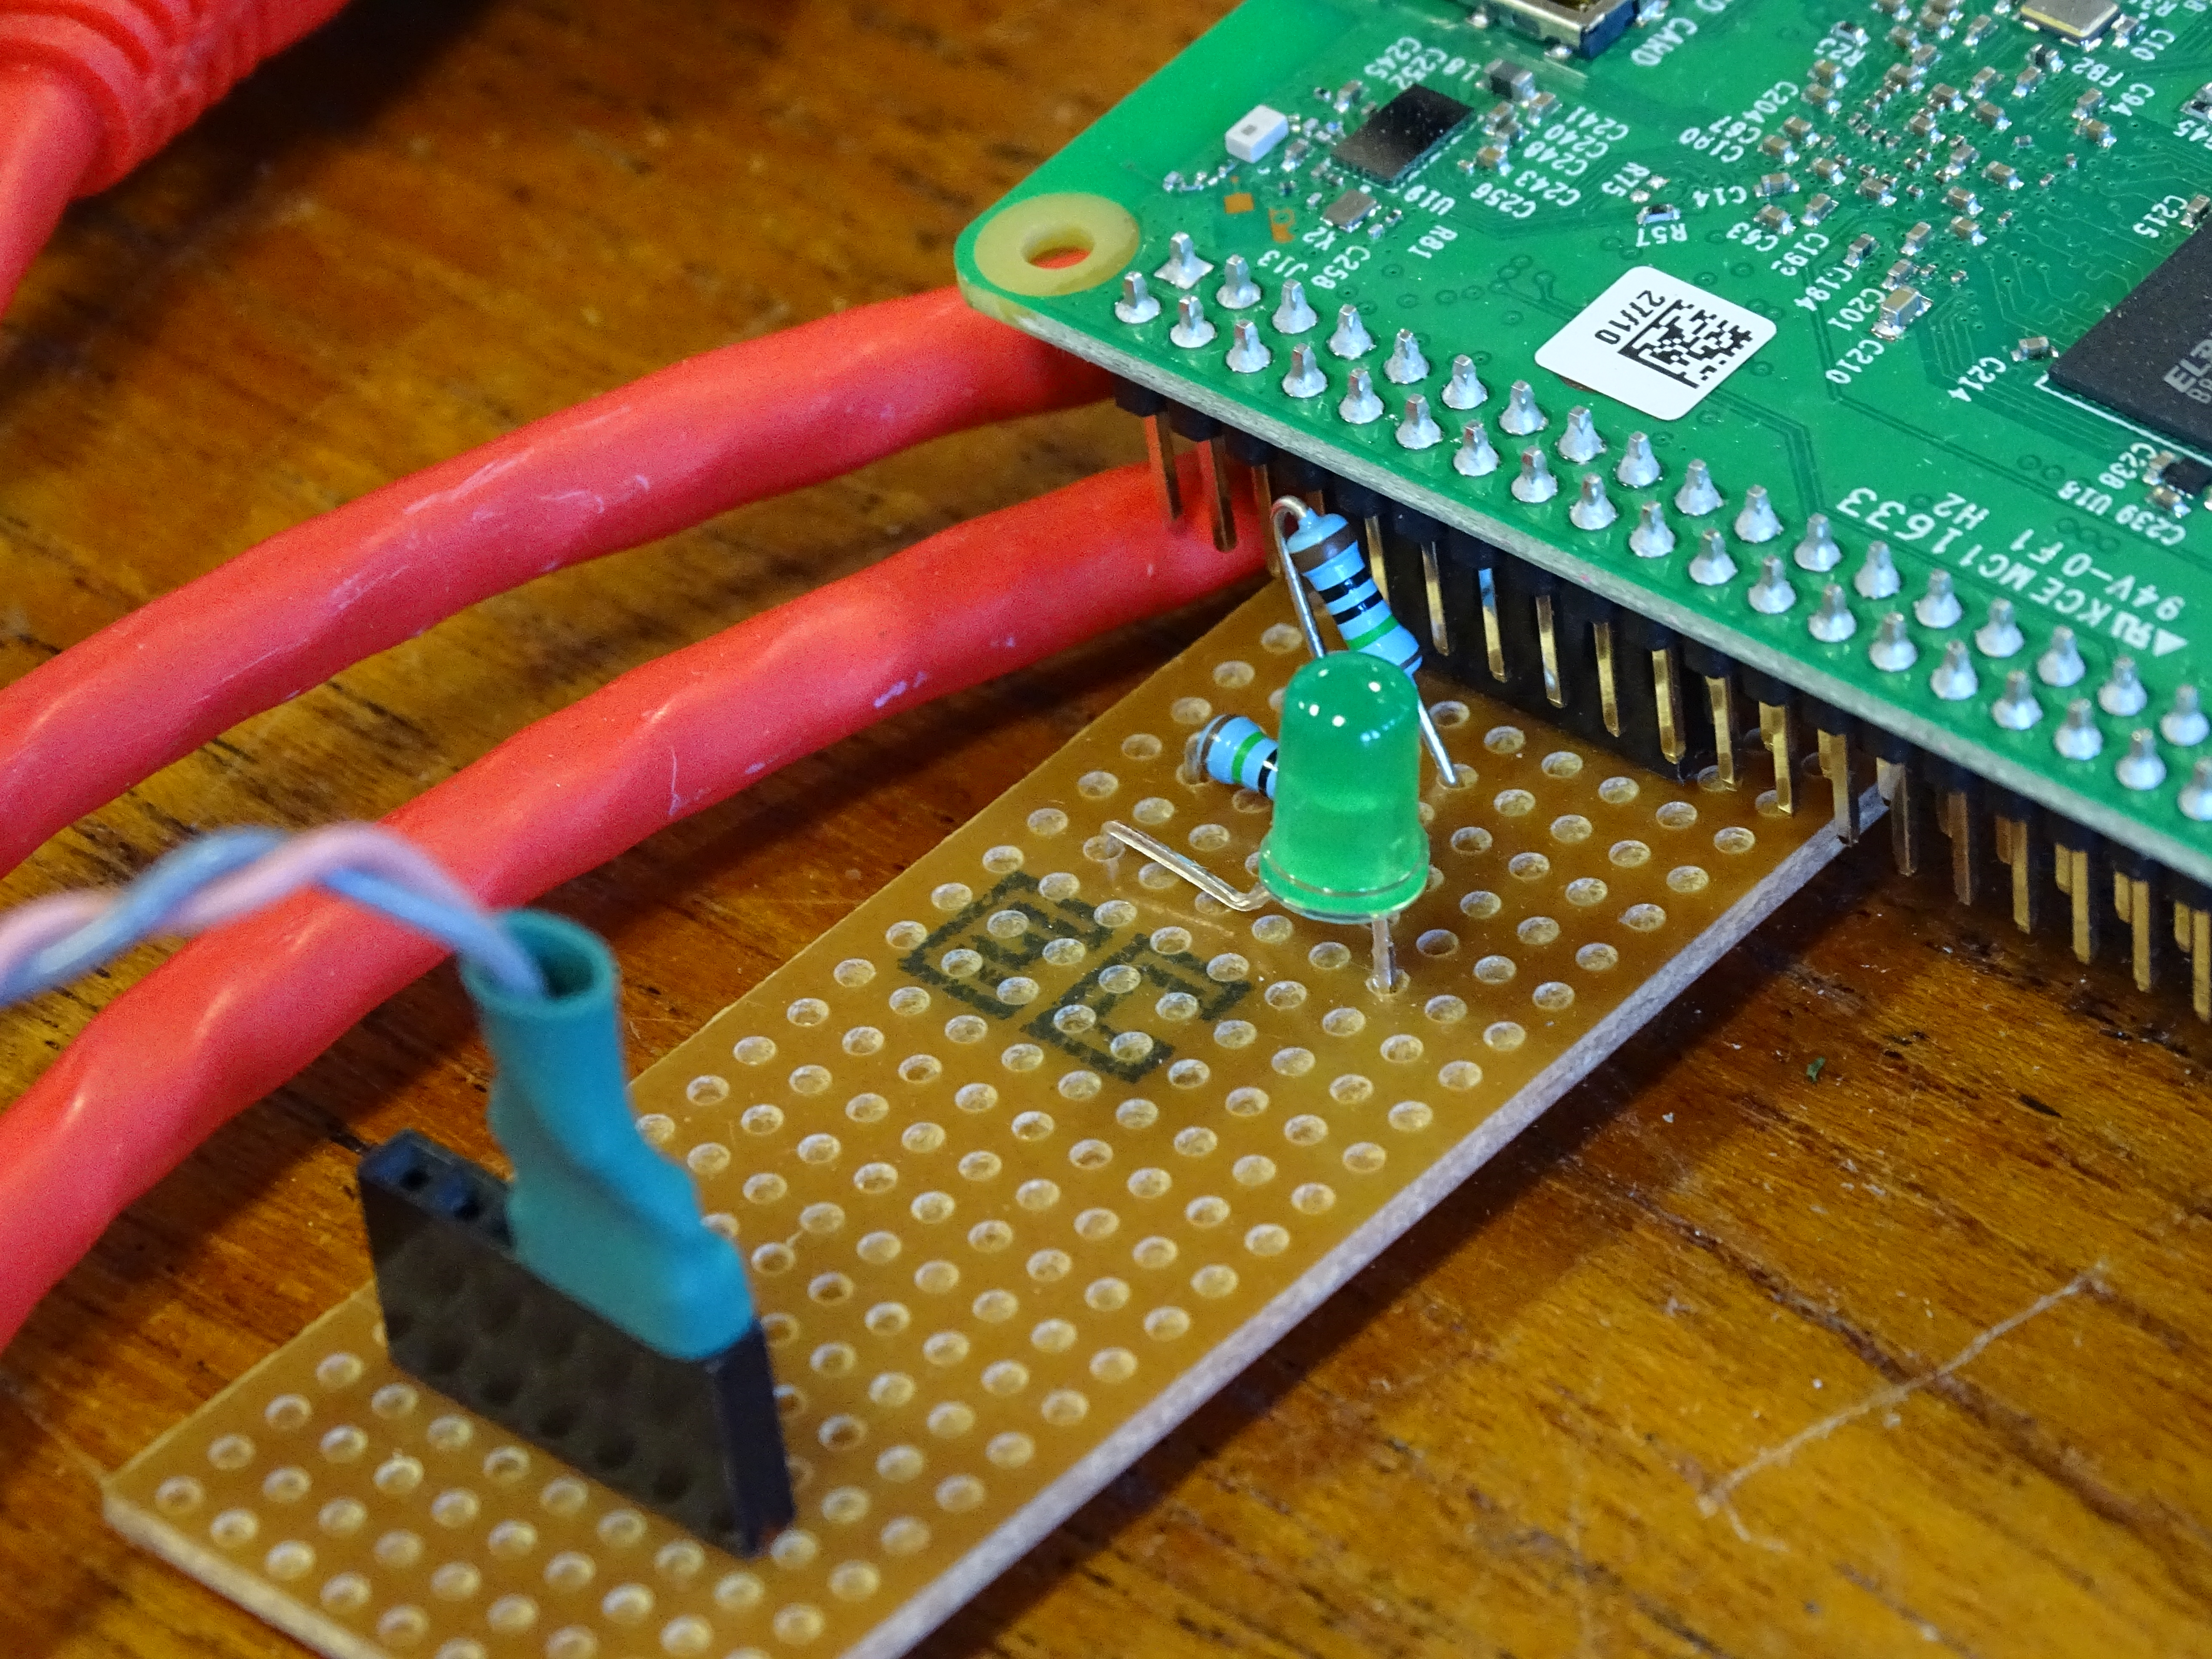
\includegraphics[width=\textwidth]{pics/meng/circuit}
                \caption{Safe caller.}
                \label{fig:circuit}
        \end{subfigure}
	\caption{Pictures of the User Interface on a monitor.}
	\label{fig:button}
\end{figure}

\subsubsection{Speech Recognition}
Thus, it was possible to know where to look for the voice, and when to start analysing. The problem was how this data would be converted to text. While offline options were considered, from prior experience with them in other coursework, they were found to be more challenging to work with. With the wealth of cloud-based options available, Microsoft Bing Cloud Speech-to-Text was chosen. This was among the various choices found through the open-source \texttt{Speech Recognition} package found for Python3.
\\\\
This package allows easy access to the cloud-service provided there is already an API key and the data is in a WAV file. This was not a problem as creating a free account for the Bing service was trivial, and that Asterisk was already recording into a WAV format. Using the function \texttt{sendToBing()}, which was based on the sample code from the package, the WAV file is sent to the online servers, and a string is returned, which contains the best guess of the voice contents.

\subsection{Metric}
The metric that was used is shown through the simple function called \texttt{callMetric()}. The argument to the function is the string of text returned from the \texttt{sendToBing()} function. Converting the string to lowercase, splitting it into words gives the list of words. These are compared with the Category A and Category B words list. The number of words from Category A and B are calculated, and according to Table \ref{tbl:metric}, the appropriate logic is used.

\section{Total Filtration System}
Combining all the above together gave the \texttt{checkNewRecording()} function. This infinite looping function has a flow as Figure \ref{fig:flow} shows.

\begin{figure}[htb]
\centering
	\begin{tikzpicture}[node distance=3cm]
	    % We start by placing the blocks
		\node [block, align=center] (start) {Start};
	    \node [block, align=center, below of=start] (lift) {Phone\\Lifted?};
		\node [block, align=center, right of=lift] (known) {Known\\Caller\\or\\Outbound};
		\node [block, align=center, below of=lift] (new) {New\\Call?};
		\node [block, align=center, left of=new] (back) {Back\\to\\Start};
		\node [block, align=center, below of=new] (wait) {Wait\\for\\Pickup};
		\node [block, align=center, below of=wait] (note) {Extract\\data\\Perform\\analysis};
		\node [block, align=center, left of=note] (risk) {Display\\risk};

	    % Once the nodes are placed, connecting them is easy.
		\draw [draw,->] (start) -- node[align=center, right] {Yes} (lift);
	    \draw [draw,->] (lift) -- node[align=center, below] {Yes} (known);
	    % \draw [->] (lift) to [bend right=45] node[align=center, left] {No} (new);
		\draw [->] (lift) to node[align=center, right] {No} (new);
		\draw [->] (new) to node[align=center, above] {No} (back);
		\draw [->] (new) to node[align=center, left] {Yes} (wait);
		\draw [->] (back.north) |- node[align=center] {} (start.west);
		\draw [->] (wait) to node[align=center, left] {Yes} (note);
		\draw [->] (wait) -| node[align=center, left] {Timeout} (back);
		\draw [->] (note) to node[align=center, above] {Yes} (risk);
		\draw [->] (known) to [in=-50,out=-130,loop, distance=3cm] node[align=center, below] {Phone in use} (known);
		\draw [->] (risk) to [in=-50,out=-130,loop, distance=3cm] node[align=center, below] {Phone in use} (risk);
		\draw [->] (known.north) |- node[align=center, right] {Call ends} (start.east);
		\draw [->] (risk) to [bend left=90] node[align=center, left] {Call ends} (back);

	\end{tikzpicture}
	\caption{\texttt{checkNewRecording()} function flow.}
	\label{fig:flow}
\end{figure}

The functions \texttt{callMetric()} and \texttt{sendToBing()} worked without a hitch. However, \texttt{checkNewRecording()} itself had an issue. Python3 had difficulty opening the WAV file as it was being edited by Asterisk. However, the system could not wait until the recording was done, and there was no easy to have recordings end midway through calls. Curiously, the raw binary data was already in the file. It was discovered that the headers were not complete in the file while Asterisk was recording.
\\\\
To get around this, the raw binary data was extracted from the file and placed into a WAV file container using Python3. This allowed the headers to be completed as the WAV writing functions from the package \texttt{wave} in Python3 automatically completed the headers. Once this was implemented correctly, the audio extraction worked correctly.
\\\\
Only 14.5 seconds of data are sent to Bing for two reasons. Firstly, it was a limitation of the free service that only 15 second sound clips are processed. Secondly, the call metric needs to be returned before too much of the call has passed.

\section{Display}
All the information from the voice analysis and reverse Turing test needs to be conveyed to the user somehow. From the Design section, the simple solution of large text on colourful backgrounds was selected. To do this, an HTML-based solution was used. Figure \ref{fig:displays} shows the final outcome.

\begin{figure}[htb]
	\captionsetup[subfigure]{position=b}
        \centering
        \begin{subfigure}{0.47\textwidth}
                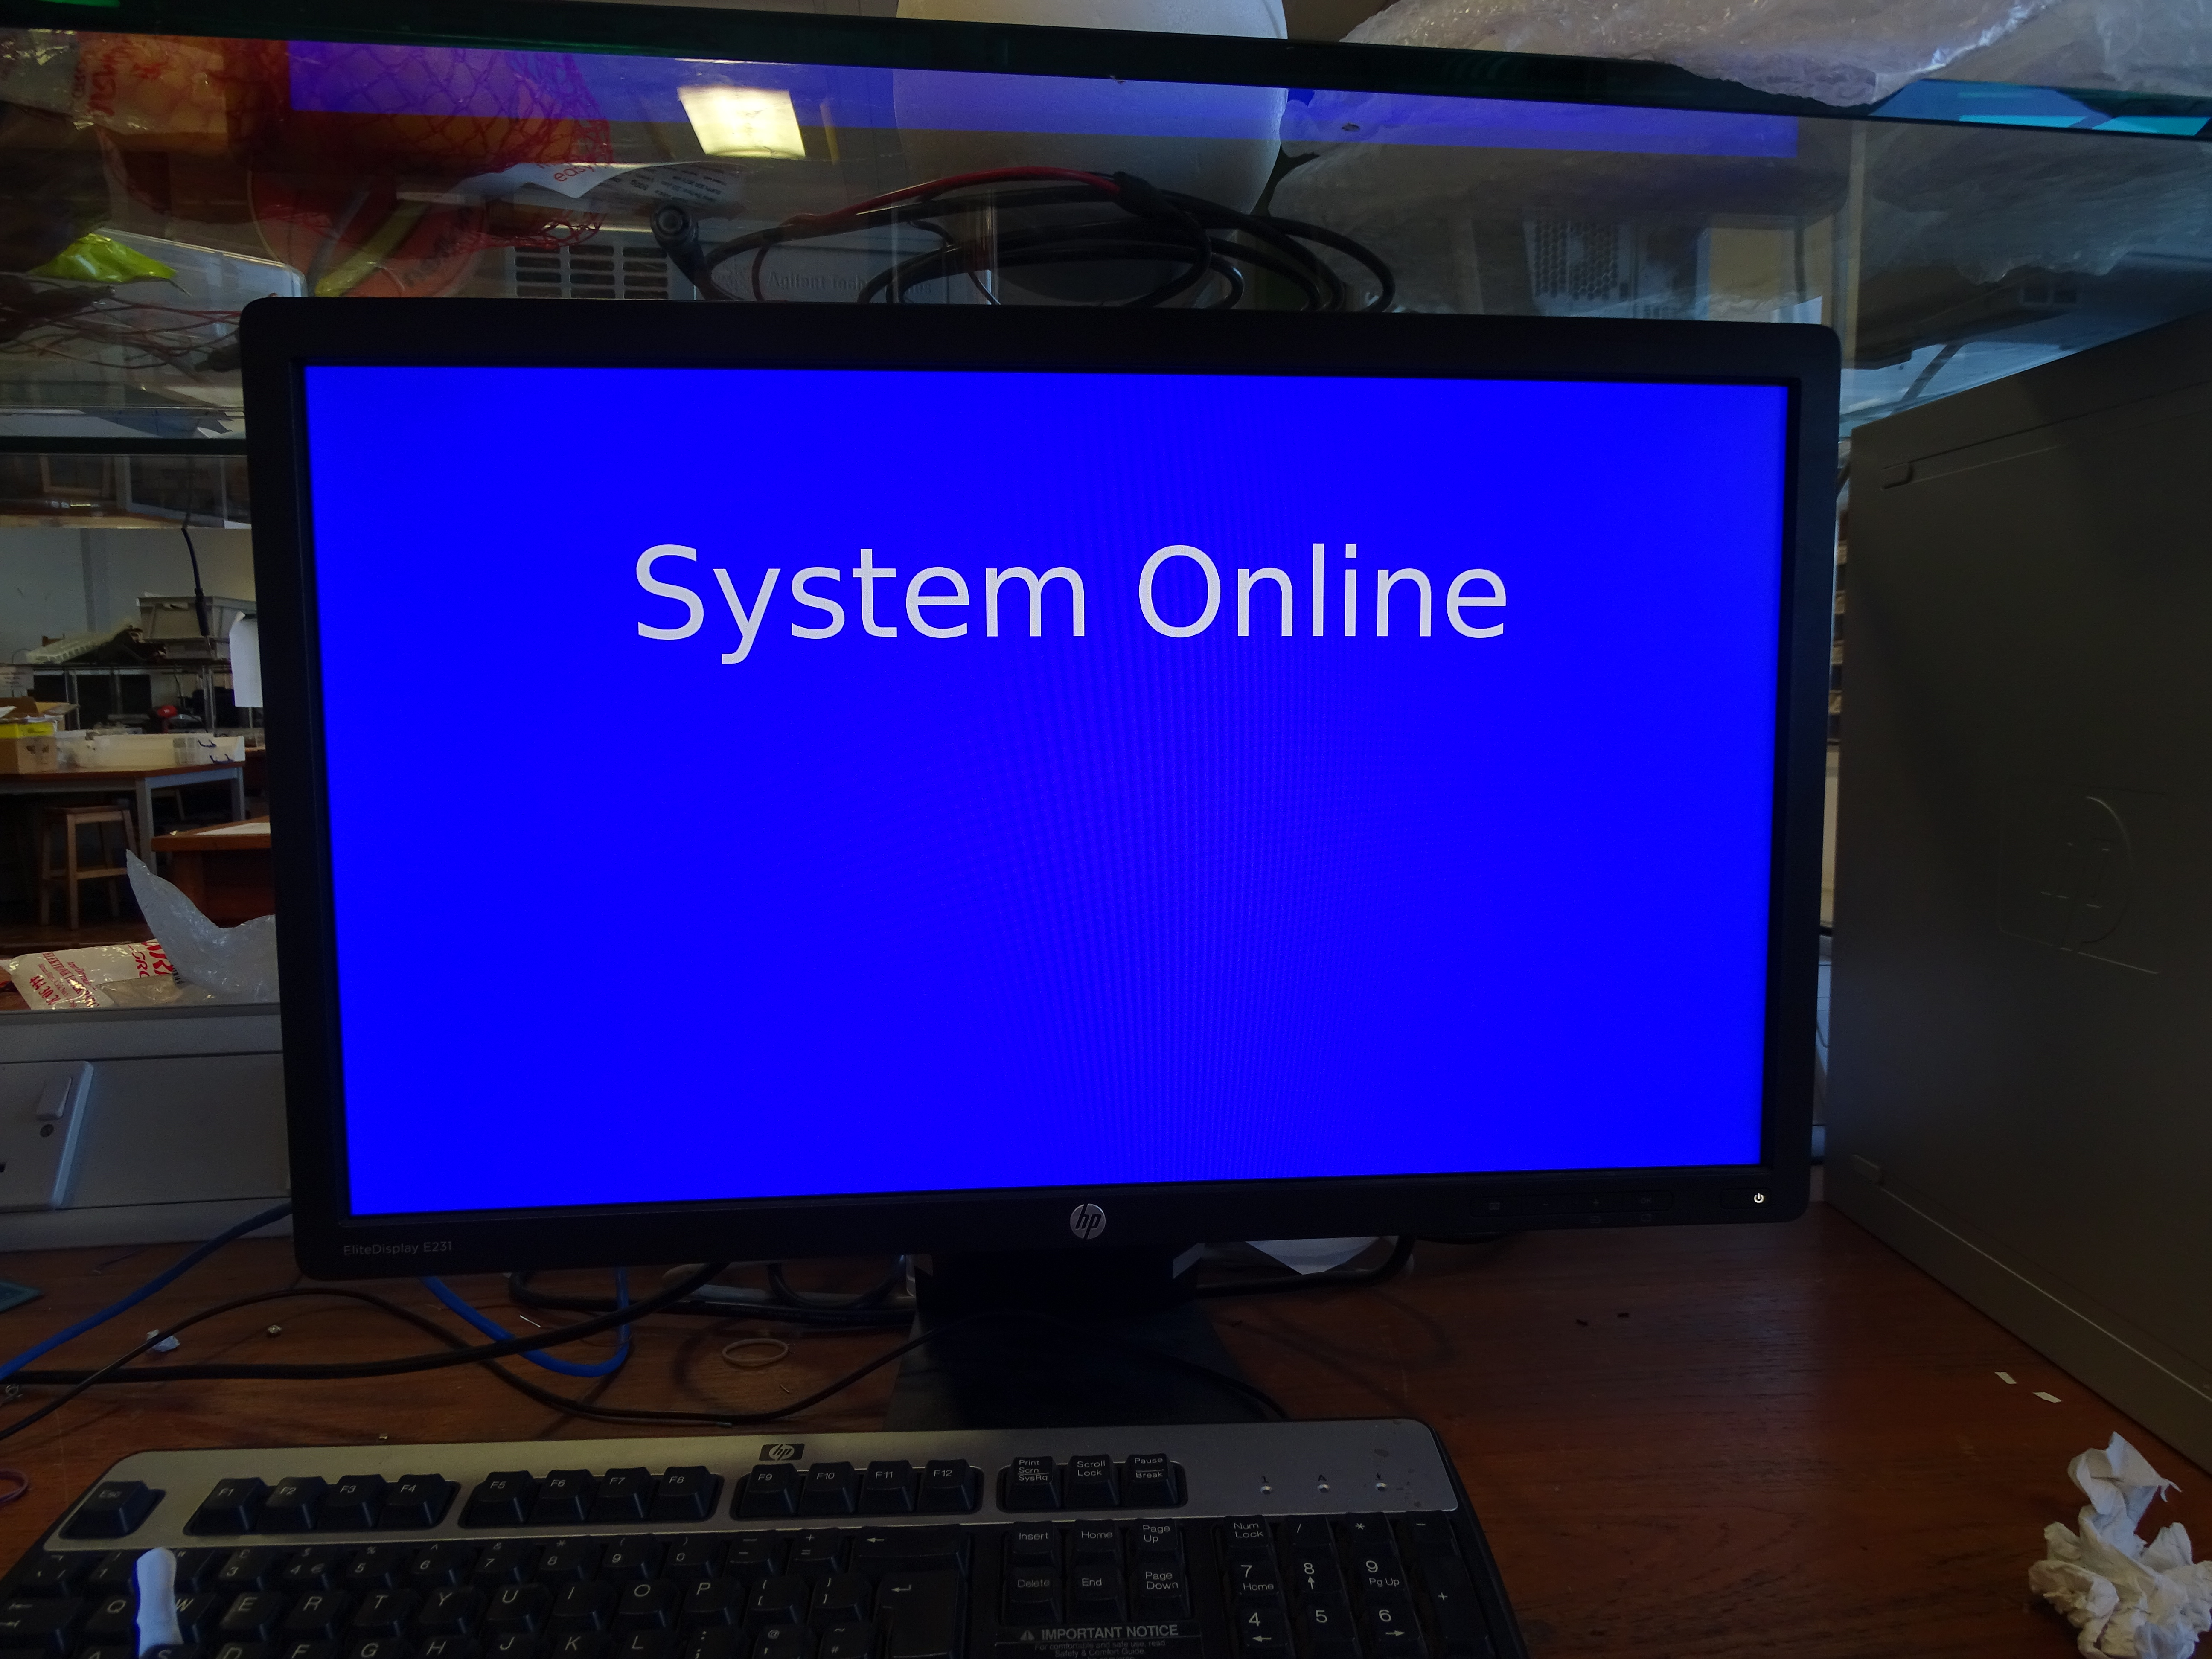
\includegraphics[width=\textwidth]{pics/meng/monitor1}
                \caption{Normal operation.}
                \label{fig:display1}
        \end{subfigure}
        ~
		\begin{subfigure}{0.47\textwidth}
                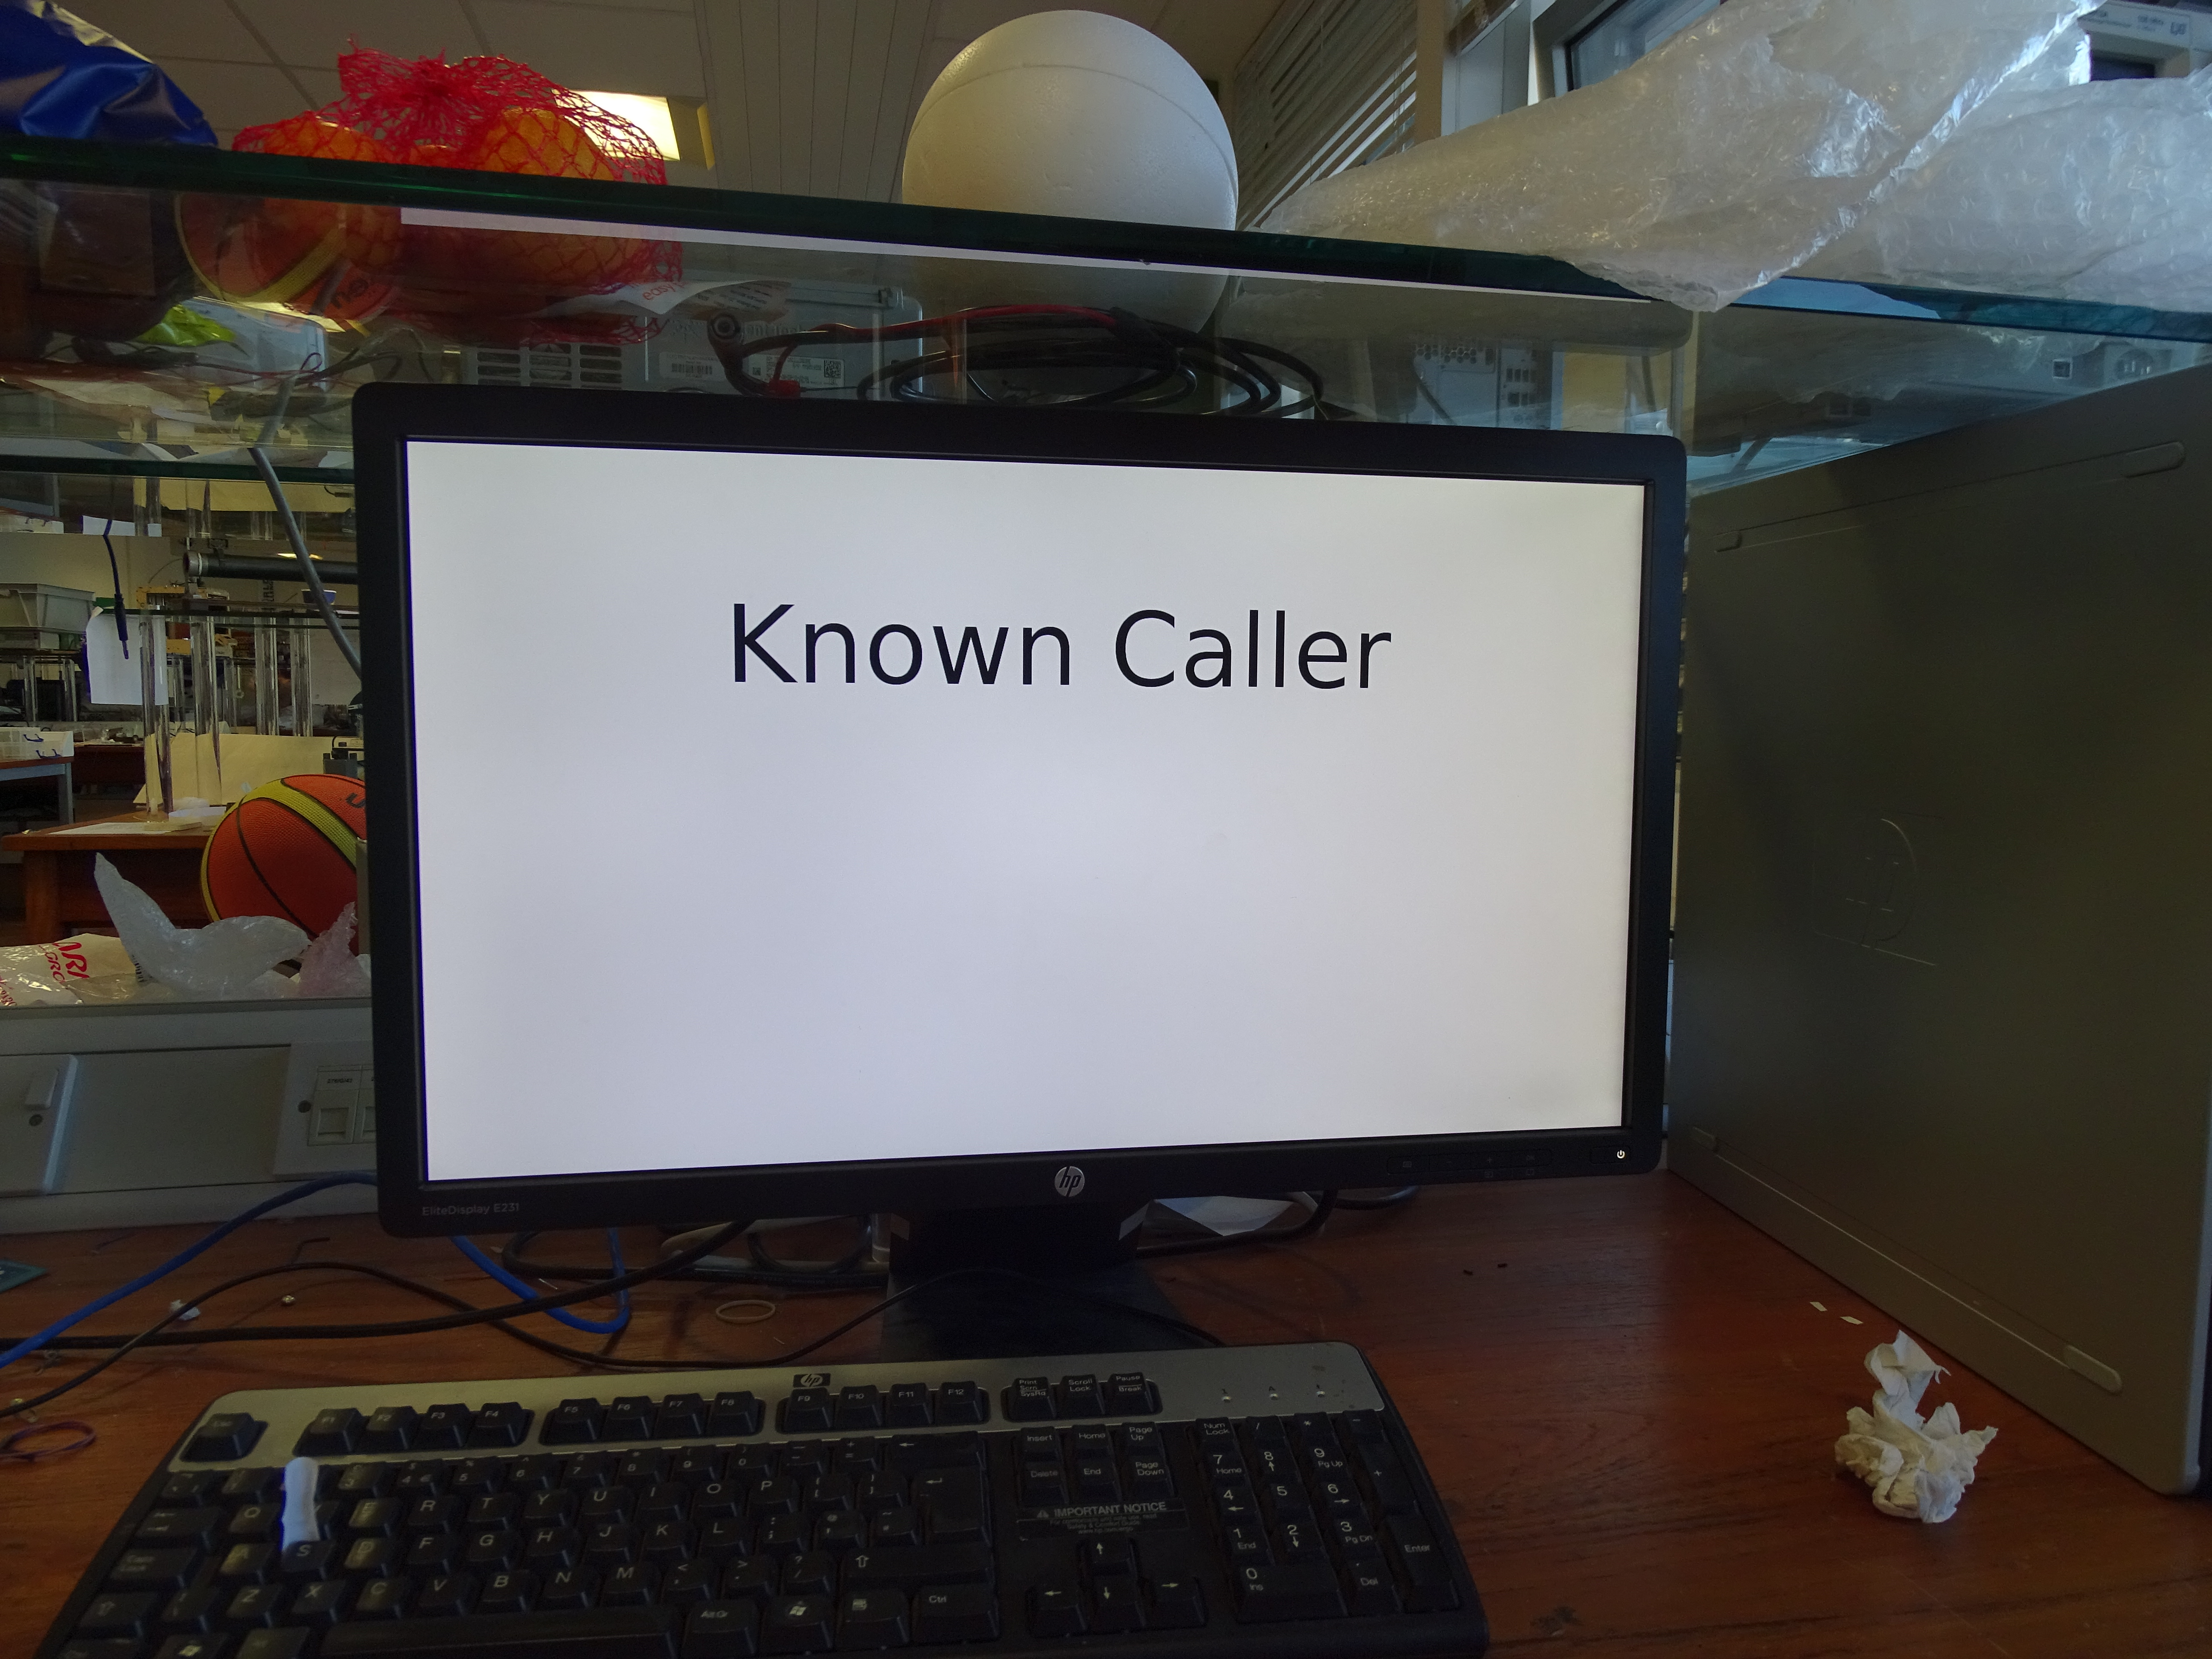
\includegraphics[width=\textwidth]{pics/meng/monitor2}
                \caption{Safe caller.}
                \label{fig:display2}
        \end{subfigure}
	\caption{Pictures of the User Interface on a monitor.}
	\label{fig:displays}
\end{figure}

\subsection{Webpage and Server}
Exploring some simple Python3 options for a website yielded the \texttt{Flask} package. This simple server system runs in Python3 with the advantage of integrating with \texttt{Jinja2}. This package allowed templates of webpages to be completed at the point of transmission, integrating conditionals, and being able to receive variables from the script. To convert the information into webpages, the concept of states was used. The full list of states chosen were as follows:

\begin{enumerate}
	\item Normal Functioning
	\item Known Caller
	\item Incoming Unknown Caller
	\item Analysing Caller Data
	\item Processing Caller Data
	\item Low risk
	\item Medium risk
	\item High risk
	\item Error
\end{enumerate}

This was very much the same as the Design phase, except additional processing states were introduced both for debugging and to keep the user aware that the system was running. There was also the error state in the event that the metric did not function correctly, which would request the user to reboot the system. The states not shown in the Design phase are seen in Figure \ref{fig:statesmore}.

\begin{figure}[htb]
	\captionsetup[subfigure]{position=b}
        \centering
        \begin{subfigure}{0.45\textwidth}
                \includegraphics[width=\textwidth]{pics/state3}
                \caption{While collecting the audio.}
                \label{fig:state3}
        \end{subfigure}
        ~
        \begin{subfigure}{0.45\textwidth}
                \includegraphics[width=\textwidth]{pics/state5}
                \caption{During the call metric function.}
                \label{fig:state5}
        \end{subfigure}
		\\
		\begin{subfigure}{0.45\textwidth}
				\includegraphics[width=\textwidth]{pics/state9}
				\caption{Error.}
				\label{fig:state9}
		\end{subfigure}
	\caption{Screens showing information to the user.}
	\label{fig:statesmore}
\end{figure}

The \texttt{checkNewRecording()} function was the one in charge of setting the state of the system as it processed the data. By having the Flask server pass this value to the template, the webpage accessed at any time would be relfective of the current state of the function. To ensure that the webpage remained up to date, a simple line made the page reload every 1 second.
\\\\
Running both the \texttt{checkNewRecording()} function and the Flask server function in the same script required some threading, with each function having its own thread. This allowed a single script to run both functions, which was easier to track, and also allowed the \texttt{checkNewRecording()} function to communicate the current state to the server. While there are considerations with threading, as the information flow was strictly one-way (function to server), there was no risk of data disruption.

\subsection{Kiosk Mode and Automation Script}
To ensure that the display only included the information, the kiosk mode of Chromium was considered. Tom Hartley of the Imperial College Robotics Society (ICRS) had experience in setting up a similar display system to manage equipment purchases in the society's lab space. Kiosk mode forces the display to fullscreen the webpage, with no address bar. Combining this with a disappearing mouse, and no peripherals bar the monitor, the user is only engaged with the material on the monitor.
\\\\
Writing a Bash script that runs at login means 3 things can be done. First, the script that contains the monitoring function and the server can run automatically. Second, Chromium can be launched in Kiosk mode, and be pointed to the server. The auto page reload means the window will continue to remain updated. Third, it gives a change to set the power settings so the monitor does not sleep. Combined with automatic login on the account configured with the code all means that the user does not need to do anything to the system at boot, and everything is taken care of. 

\end{document}
